To compare two numbers we use a process that mimics the behavior of arithmetic circuits for comparing two bits binary numbers shown in 
\refFig{tra_comparator_circuit}.
\refFig{tra_comparation} shows visualization and  ABC code of the comparator process and a simple if-else statement.
The full implementation of $Compare$ processes can be found in the appendix.
\begin{figure}[H]%
\centering
\fbox{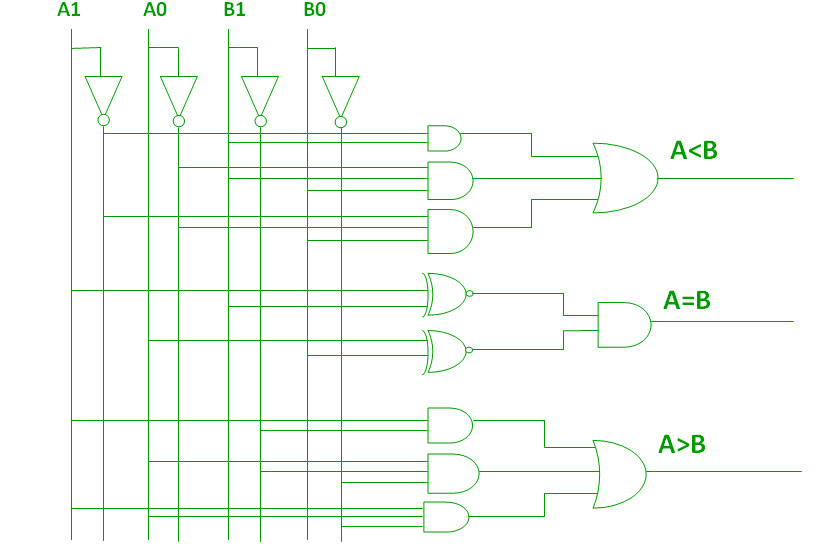
\includegraphics[keepaspectratio,width=0.85\textwidth]{./images/transformational_semantics_of_oz/comparator_circuit.png}}
\caption{comparator circuit}
\label{tra_comparator_circuit}%
\end{figure}


\begin{figure}[H]%
\centering
\subcaptionbox{Before comparation.}{\fbox{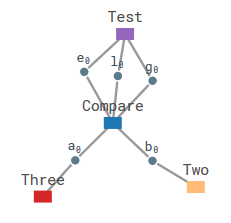
\includegraphics[keepaspectratio,width=0.45\textwidth]{./images/transformational_semantics_of_oz/comparator_before.png}}}%
\hspace{1em}%
\subcaptionbox{After comparation.}{\fbox{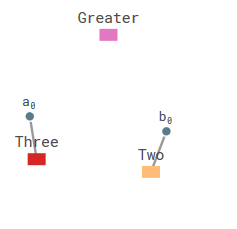
\includegraphics[keepaspectratio,width=0.45\textwidth]{./images/transformational_semantics_of_oz/comparator_after.png}}}%
\vspace{2em}
\subcaptionbox{ABC code.}{\fbox{$(\ \widehat{}\ \text{a,b,g,e,l}\ )\ (\ \text{Three}(\text{a})\ \mid\ \ \text{Two}(\text{b})\ \mid\ \ \text{Compare}(\text{a,b,g,e,l})\ \mid\ \ \text{If\_Else}(\text{g,e,l})\ )$}}%
\caption{comparation as a process}
\label{tra_comparation}%
\end{figure}
